\documentclass[11pt]{exam}
\usepackage[margin=1in]{geometry}
\pagestyle{plain}
\usepackage{amsmath,amsfonts,amssymb,amsthm,enumerate}
\usepackage{multicol}
\usepackage[]{graphicx}
\usepackage{hyperref}
\usepackage{tikz}
\usepackage{pgfplots}
\usepackage{subfigure}
\usepackage[final]{pdfpages}

\addtolength{\footskip}{2\baselineskip} % to lower the page numbers
\title{\vspace{-0.5in} Math 115\\ Worksheet Extrema Review}
\date{}


% \theoremstyle{definition}
% \newtheorem{problem}{Problem}
\renewcommand{\questionlabel}{\textbf{Problem~\thequestion.}}
\printanswers

\begin{document}
\maketitle
\vspace{-0.75in}
\section*{Local Extrema and Inflection Points}
\begin{questions}
\question (Winter 2020 Final)
  Consider the continuous function \[
    g(x) =
    \begin{cases}
      -(x^2+12x+37) e^{-x} + 17 & x \leq 0\\
      7x^3 - 21 x^2 - 168 x - 20 & x > 0
    \end{cases}
  \]
  Note that \[
    g'(x) =
    \begin{cases}
      (x+5)^2 e^{-x} & x < 0 \\
      21(x-4)(x+2) & x > 0
    \end{cases}
  \]
  \begin{parts}
  \part Find the critical points of \(g(x)\)
  \part Find the \(x\)-coordinate of all local extrema of \(g(x)\), and classify each as a local maximum
or a local minimum. Use calculus to find and justify your answers, and be sure to show enough
evidence that you have found all local extrema.
  \end{parts}
  \begin{solution}
    See \href{https://dhsp.math.lsa.umich.edu/exams/115exam3/w20/s5.pdf}{https://dhsp.math.lsa.umich.edu/exams/115exam3/w20/s5.pdf}
  \end{solution}
  \question (Fall 2019 Exam 2) % problem 3
    Suppose \(q(x)\) is a differentiable function defined for all real numbers \(x\). The derivative
and second derivative of \(q(x)\) are given by 
\begin{center}
  \(q'(x) = x^{2/3}(x - 3)^{5/3}(x + 5)\) and
  \(q''(x) = \frac{10(x - 3)^{2/3}(x - 1)(x + 3)}{3x^{1/3}}\)
\end{center}
\begin{parts}
\part Find the \(x\)-coordinates of all critical points of \(q(x)\). If there
  are none, write none.
\part Find the \(x\)-coordinates of all critical points of
  \(q'(x)\). If there are none, write none.
\part Find the \(x\)-coordinates of all local maxima and local minima
  of \(q(x)\). If there are non of a particular type, write none. Use
  calculus to find and justify you answers, and be sure to show enough
  evidence to demonstrate that you have found all local extrema.
\part Find the \(x\)-coordinates of all inflection points of
  \(q(x)\). If there are none, write none.
Use calculus to find and justify your answers, and be sure to show enough evidence to
demonstrate that you have found all inflection points.
\end{parts}
\begin{solution}
     See \href{https://dhsp.math.lsa.umich.edu/exams/115exam2/f19/s3.pdf}{https://dhsp.math.lsa.umich.edu/exams/115exam2/f19/s3.pdf}
    \end{solution}
\vspace{-0.25in}
\section*{Global Extrema}
\vspace{-0.25in}
\question (Winter 2019 Exam 3)
  Consider the continuous function \[
    f(x) =
    \begin{cases}
      -2 - \ln(x+2) & -2 < x \leq -1 \\
      x2^{-x} & x > -1
    \end{cases}
  \]
  and its derivative \[
    f'(x) =
    \begin{cases}
      - \frac{1}{x+2} & -2 < x < -1 \\
      2^{-x}(1-x\ln(2)) & x > -1 
    \end{cases}
  \]
  \begin{parts}
  \part Find all critical point(s) of \(f(x)\). Write none if there are none.
  \part Find the \(x\)-coordinate of all global maxima and global
    minima of \(f(x)\) on its domain \((-2,\infty)\). For each, write none if there are none. You must use calculus to find your answers,
and be sure to show enough evidence to fully justify your answers
  \end{parts}
  \begin{solution}
    See \href{https://dhsp.math.lsa.umich.edu/exams/115exam3/f19/s10.pdf}{https://dhsp.math.lsa.umich.edu/exams/115exam3/f19/s10.pdf}
  \end{solution}
\question (Winter 2016 Exam 2) % problem 9
  Consider a continuous function \(T\) with the following properties.
  \begin{itemize}
  \item \(T(v)\) is defined for all real numbers v.
  \item The critical points
    of \(T(v)\) are the four points \(v = 3, v = 5, v = 7\), and \(v = 8\). (\(T(v)\)
    has no other critical points.)
  \end{itemize}
  Some values of \(T\) are shown in the following table:\\
  \begin{tabular}{|c|c|c|c|c|c|c|}
    \hline
    \(v\)&0&3&5&7&8&10\\
    \hline
    \(T(v)\)&21&9&13&19&11&21\\
    \hline
  \end{tabular}

  For each of a.-f. below, use the answer blank provided to list all the values \(v\) at which \(T(v)\) attains the specified global extremum. If there is not enough information provided to give an answer, write “not enough info”. If \(T(v)\) does not attain the specified global extremum on the specified interval, write “none”.

  For what value(s) \(v\) does \(T(v)\) attain its... 
  \begin{parts}
  \part global minimum on the interval \(0 \leq v \leq 10\)?
  \part global maximum on the interval \(0 \leq v \leq 10\)?
  \part global minimum on the interval \(0 < v < 10\)?
  \part global maximum on the interval \(0 < v < 10\)?
  \part global minimum on the interval \((-\infty,\infty)\)?
  \part global maximum on the interval \((-\infty,\infty)\)?
  \end{parts}
  \begin{solution}
    See \href{https://dhsp.math.lsa.umich.edu/exams/115exam2/w16/s9.pdf}{https://dhsp.math.lsa.umich.edu/exams/115exam2/w16/s9.pdf}
  \end{solution}
\question (Fall 2018 Exam 2) Consider the function \[
    f(x) =
    \begin{cases}
      4-x-x^{\frac{2}{3}} & -8 \leq x \leq 0\\
      5xe^{-0.5x} + 4 & x > 0
    \end{cases}
    \text{ and its derivative }
    f'(x) =
    \begin{cases}
      \frac{2+3x^{\frac{1}{3}}}{-3x^{\frac{1}{3}}}  & -8 < x < 0 \\
      5(1-0.5x) e^{-0.5x} & x > 0
    \end{cases}
  \]
Find the x-coordinates of the global maximum and the global minimum of the function f(x) for \(x \geq -8\). If
one of them does not exist, write none in the answer line below. Use calculus to find your answers, and be
sure to show enough evidence that the point(s) you find are indeed global extrema.
\pagebreak
\section*{Optimization}
\vspace{-0.25in}
\question A garden store plans to build a large rectangular
sign on the interior wall at one end of their green-
house. For x and y in meters, the curved roof of the
greenhouse is described by the function \[
  y = 5 - \frac{5}{16} x^2 \text{ for } -4 \leq x \leq 4
\]
The curve is graphed below. The shaded rectangle is one possible sign
that could be built.
\begin{center}
  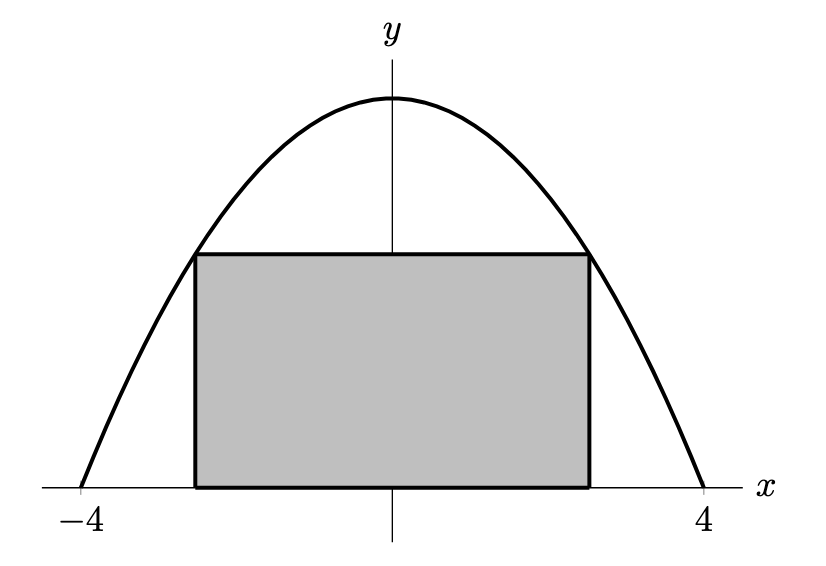
\includegraphics[scale=0.5]{Figures/greenhouse}
\end{center}

Find the width and height of the sign with the maximum area. Use
calculus to find your answers, and be sure to show enough evidence
that the values you find do in fact maximize the area.
\begin{solution}
  See \href{https://dhsp.math.lsa.umich.edu/exams/115exam3/f19/s6.pdf}{https://dhsp.math.lsa.umich.edu/exams/115exam3/f19/s6.pdf}
\end{solution}
\section*{Putting it all together}
\question (Winter 2016 Exam 2) % problem 10
Let \(j(t)\) be a differentiable function with domain \((0, \infty)\) that satisfies all of the following:
\begin{itemize}
\item \(j(5) = 0\)
\item \(j(t)\) has exactly two critical points
\item \(j(t)\) has a
  local maximum at \(t = 5\)
\item \(j(t)\) has a local minimum at \(t = 9\)
\item \(\lim_{t \to 0^+} j(t) = -\infty\)
\item \(\lim_{t \to \infty} j(t) = 0\)
\end{itemize}
\begin{parts}
\part Circle all of the following intervals on which \(j'(t)\) must
  always be negative. \[
    (0,2) \qquad (2,5) \qquad (5,9) \qquad (9,\infty)
  \]
\part Find all the values of \(t\) at which \(j(t)\) attains global extrema on the interval \([1, 9]\). If
not enough information is provided, write not enough info. If there are no such values of \(t\),
write none.
\part Find all the values of \(t\) at which \(j(t)\) attains global extrema on its domain. If not
enough information is provided, write not enough info. If there are no such values of \(t\), write
none.
\end{parts}
\begin{solution}
  See \href{https://dhsp.math.lsa.umich.edu/exams/115exam2/w19/s10.pdf}{https://dhsp.math.lsa.umich.edu/exams/115exam2/w19/s10.pdf}
\end{solution}
\ifprintanswers
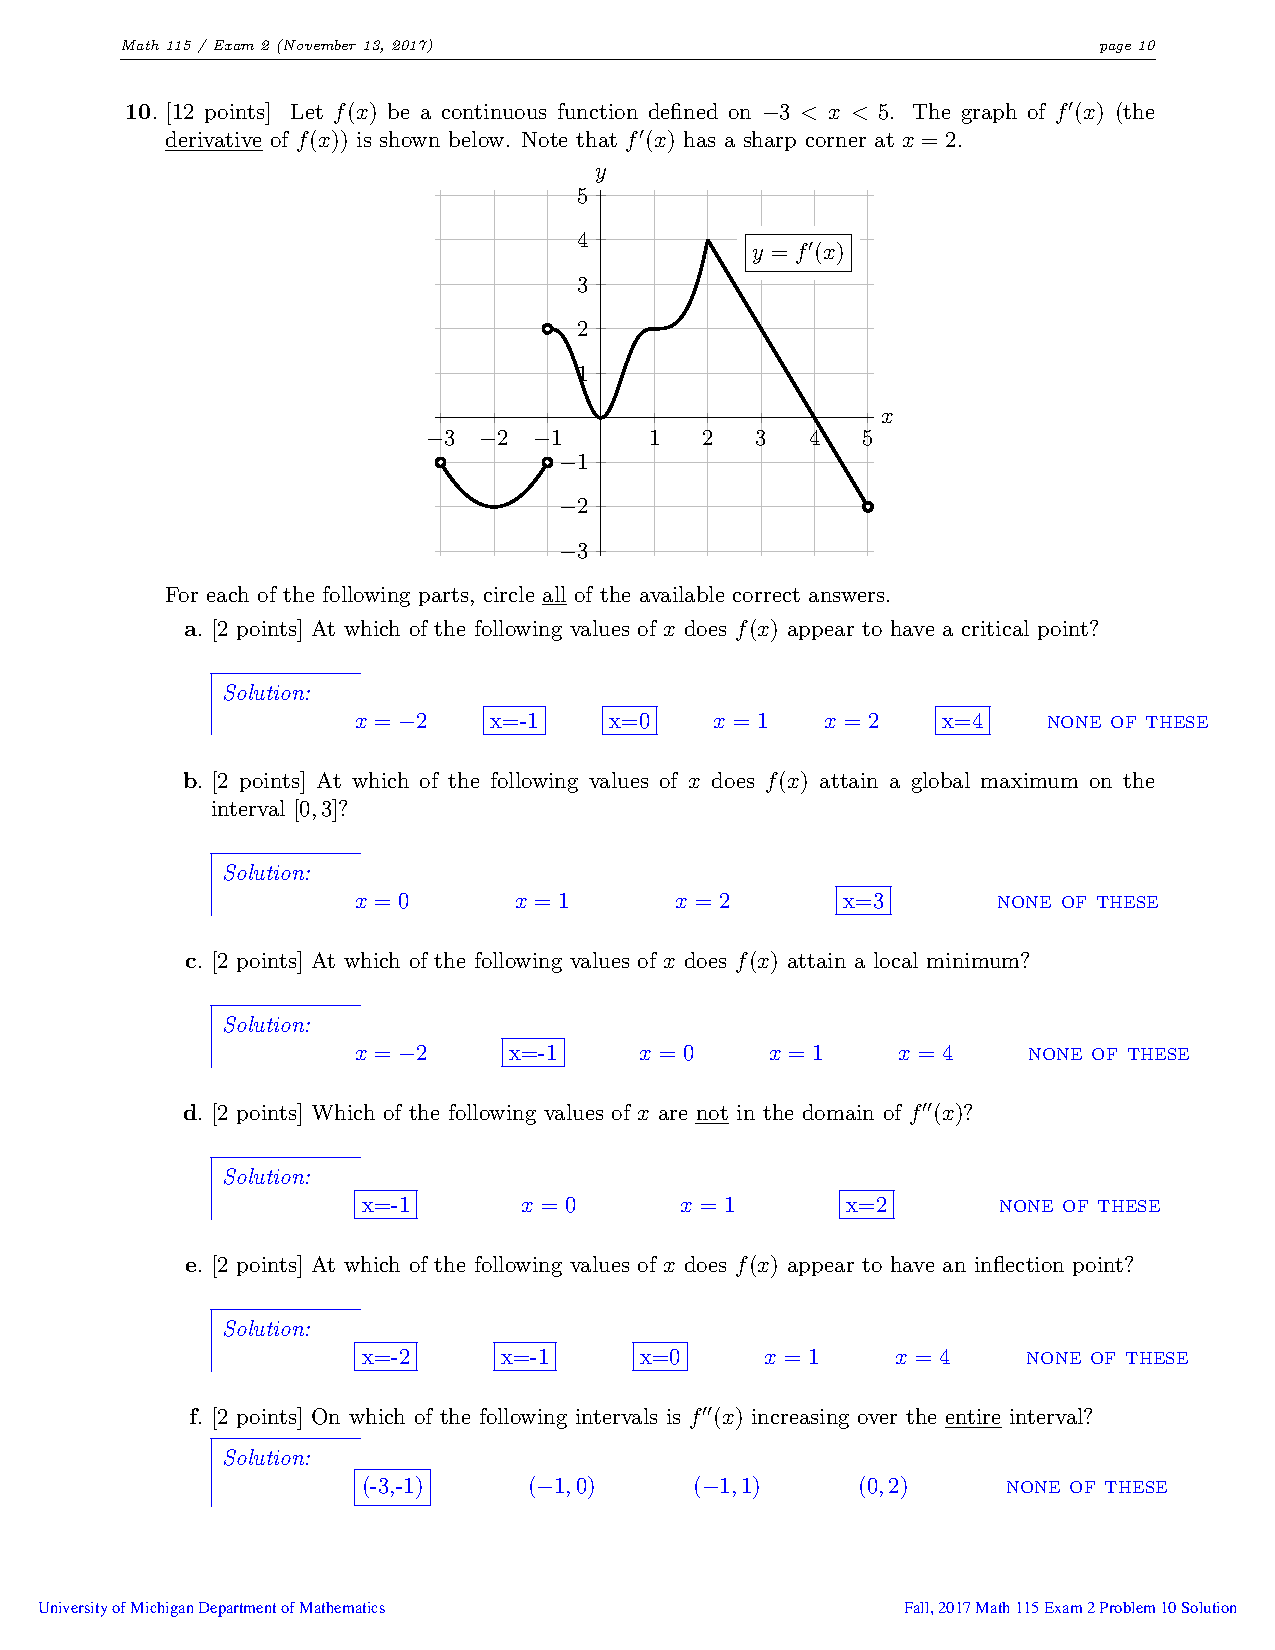
\includepdf[pages=-,pagecommand={}]{Figures/s10.pdf}
\else
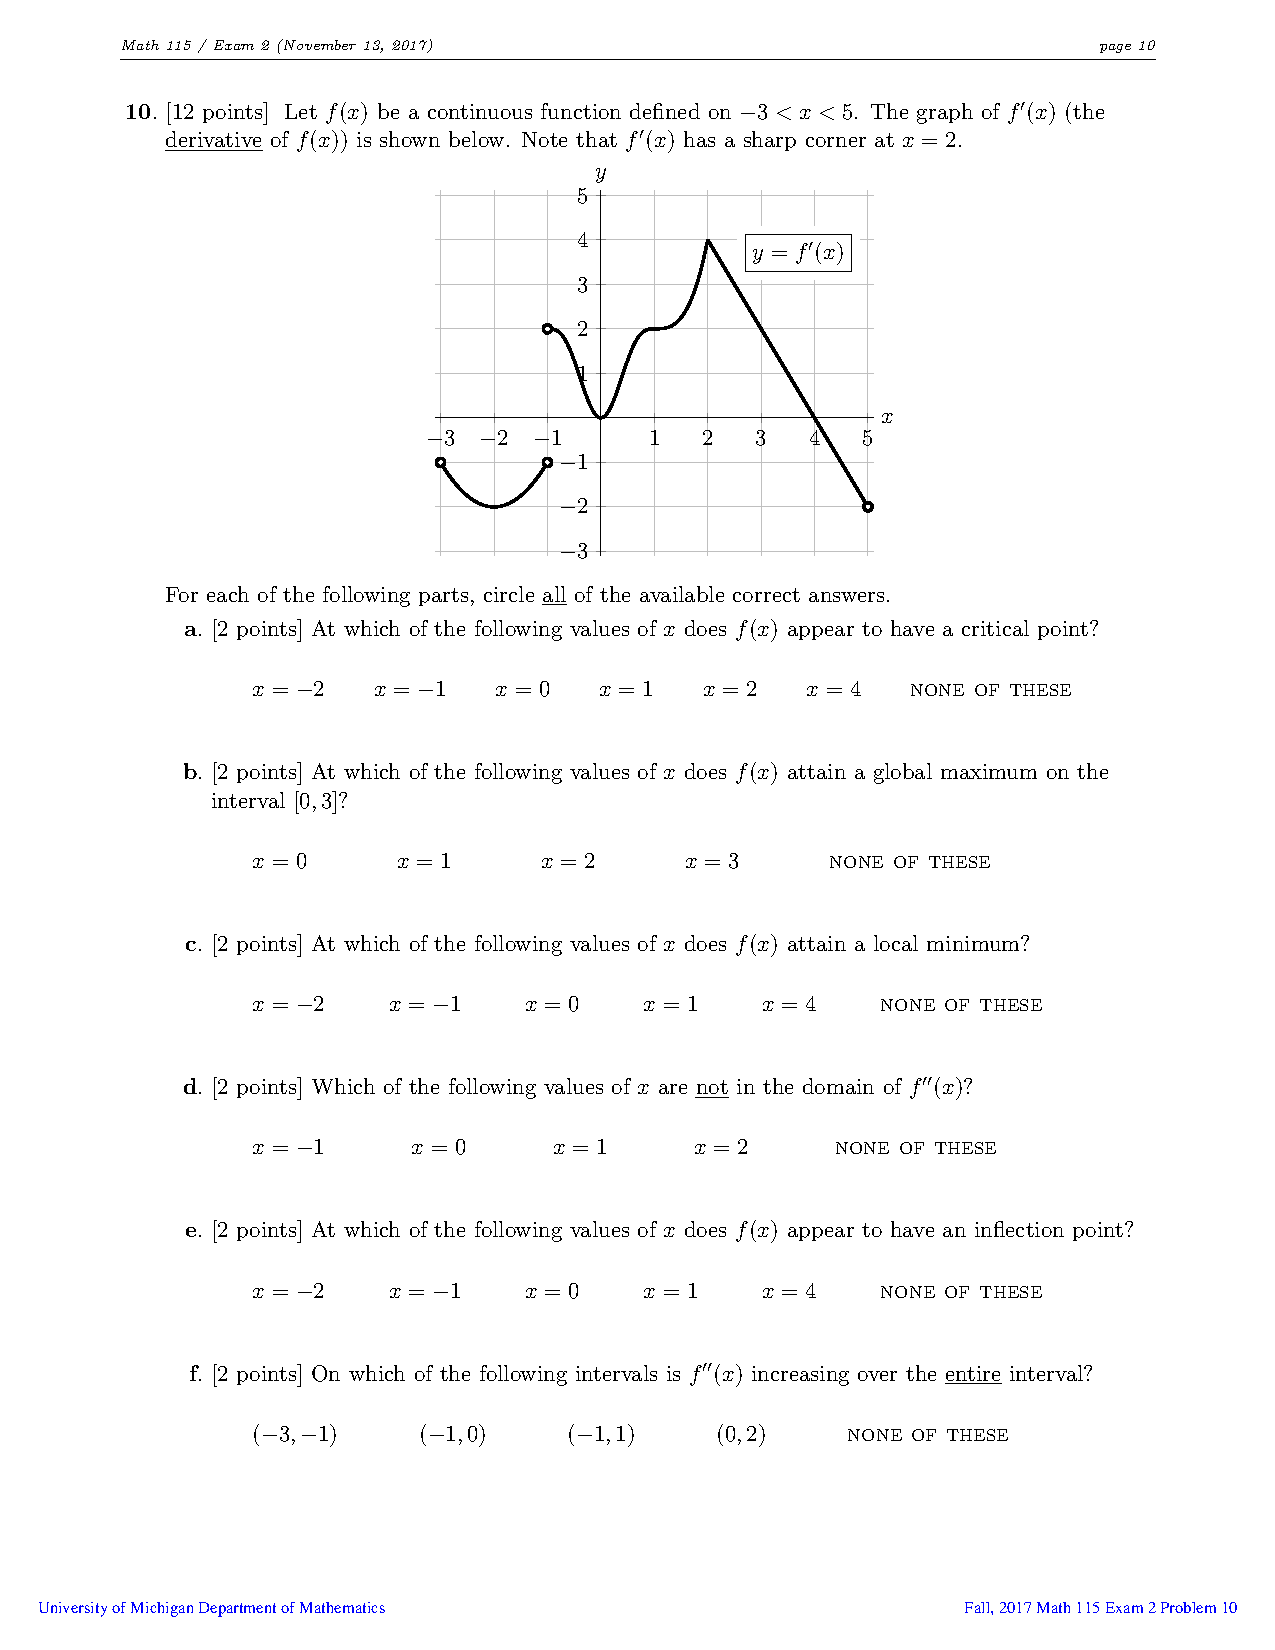
\includepdf[pages=-,pagecommand={}]{Figures/p10.pdf} 
\fi
\end{questions}
\end{document}
%%% Local Variables:
%%% mode: latex
%%% TeX-master: t
%%% End:
